
At the most general it might be expected to start in the same way as Peierls, by bringing together two half crystals as shown in \autoref{fig:semi_infinite_crystals} and simply allowing the structure to relax, leaving all the atomic positions as free variables. If the dislocation is indeed a stable defect then it will form and the energy found, however with no constraints applied at all the dislocation would always relax to its low energy equilibrium position, and even if it did not a global optimiser that allowed large enough deviations from the initial configuration might remove the dislocation entirely and form a small perfect crystal. Therefore even in a very general approach appropriate constraints must be employed. Additionally the tractability of optimising the positions of many thousands if not millions of atoms for every value of $\alpha$ mean that a less general approach might be necessary. 

To incorporate constraints and parametrise the configuration the model could employ a displacement field. For a given value of $\alpha$ there will be some initial configuration of atoms defined by two half crystals brought together at a slip plane with some relative displacement between them defined by the Burgers vector. The core of the dislocation is taken to be the line at $x,y = 0$. The position of the core with respect to the lattice of the half crystals is defined by $\alpha$, usually with $\alpha=0$ defining the configuration in which the extra half-plane of atoms aligns with the dislocation core, as shown in \autoref{fig:joined_half_crystals}. 

The final (in the sense of ready to be evaluated energetically rather than optimised) configuration is these initial positions plus an array of displacements defined by some displacement field, $\bm{\delta}(x_0, y_0, z_0)$, i.e.
\begin{equation}
\mathbf{r}_i = \mathbf{r}_i^0 + \bm{\delta}(\bm{r}_i^0)
\end{equation}
where $\mathbf{r}_i$ is the position vector defining the final position of the $i$th atom, $\mathbf{r}_i^0$ is the vector defining the initial position of the $i$th ion and $\bm{\delta}$ is a vector displacement field.


%%%%%%%%%%%%%%%%%%%%%%%%%%%%%%%%%%%%%%%%%%%%%%%%%%%%%%%%%%%%%%%%%%%%%%%%%%%5
%
%                      Initial half crystals
%
%%%%%%%%%%%%%%%%%%%%%%%%%%%%%%%%%%%%%%%%%%%%%%%%%%%%%%%%%%%%%%%%%%%%%%%%%%%%%%
\subsection{Defining the initial atomic positions}


Firstly we must define the initial positions of the atoms in the half crystals. To create a crystal conveniently oriented with respect to the Cartesian reference axes and the crystal slip system unconventional unit cells were defined. Directions and planes defined relative to the unconventional or dislocation cell will be marked prime, e.g. $[100]'$. The Burgers vector $\mathbf{b}$ is taken to be the $[100]'$, the shortest slip plane normal that is a full lattice vector is taken to be $[010]'$ and the $[001]'$, parallel to the line vector $\mathbf{l}$, is the shortest lattice vector that is perpendicular to both the Burgers vector and the slip plane normal and its sign is such that the axes are right handed. Filling space by convolving a motif and a lattice defined according to these axes is convenient because most of the mathematical results of dislocation theory, stress and strains fields etc, are defined taking $x$, $y$ and $z$ parallel to $[100]'$, $[010]'$, $[001]'$ respectively.

For example the \ce{NaCl} <1\={1}0>\{110\} slip system gives a new unit cell aligned with the slip system:

\begin{equation*}
\begin{aligned}[c]
{[100]}' &=\, ^{1}\!/_{2} [110]   \\
{[010]}' &=\, ^{1}\!/_{2} [1\overline{1}0]   \\
{[001]}' &=\, [001]   
\end{aligned}[c]
\qquad
\begin{aligned}[c]
&\parallel \mathbf{b} \\
&\parallel \mathbf{d} \\
&\parallel \mathbf{l}
\end{aligned}
\end{equation*}



This tetragonal unit cell contains 2 lattice points so the motif cannot be simply rotated from the conventional case, a new motif is
$$
motif = \begin{pmatrix}
0 & 0 & 0 & +1 \\
^{1}\!/_{2} & ^{1}\!/_{2} & ^{1}\!/_{2} & +1 \\
0 & 0 & ^{1}\!/_{2} & -1 \\
^{1}\!/_{2} & ^{1}\!/_{2} & 0 & -1 \\
\end{pmatrix}
$$
where a $+1$ in the final column denotes a sodium ion and a $-1$ denotes a chloride ion.



\begin{figure}
\centering


    \begin{subfigure}{0.55\textwidth}
    \centering
    \includegraphics[width=\textwidth]{NaCl}
    \caption{The conventional unit cell of sodium chloride with the salient slip directions and plane normals highlighted. \label{fig:NaCl_conventional_cell_slip_system_marked}}
    \end{subfigure}

    \begin{subfigure}{0.4\textwidth}
    \centering
    \includegraphics[height=2.0in]{NaCl_110_110_w_axes}
    \caption{The sodium chloride unit cell best aligned with the <110>\{1\={1}0\} slip system. \label{fig:NaCl_110_110_unit_cell}}
    \end{subfigure}
    ~
    \begin{subfigure}{0.4\textwidth}
    \centering
    \includegraphics[height=2.5in]{NaCl_110_001_w_axes}
    \caption{The sodium chloride unit cell best aligned with the <110>\{001\} slip system. \label{fig:NaCl_110_001_unit_cell}}
    \end{subfigure}

\caption{Possible unit cells for sodium chloride showing the conventional unit cell and two unconventional unit cells with the new crystallographic axes aligned to slip system, i.e. the Burgers vector and slip plane normal.\label{fig:unconventional_NaCl_unit_cells}}
\end{figure}






Similarly the \ce{NaCl} <1\={1}0>\{001\} slip system is defined by the unit cell:

\begin{equation*}
\begin{aligned}[c]
 {[100]}' &=\, ^{1}\!/_{2} [110] \\
 {[010]}' &=\,  [001] \\
 {[001]}' &=\; ^{1}\!/_{2} [1\overline{1}0] \\
\end{aligned}
\qquad
\begin{aligned}[c]
&\parallel \mathbf{b} \\
&\parallel \mathbf{d} \\
&\parallel \mathbf{l}
\end{aligned}
\end{equation*}


and a possible new motif is 
$$
motif = \begin{pmatrix}
0 & 0 & 0 & +1 \\
^{1}\!/_{2} & ^{1}\!/_{2} & ^{1}\!/_{2} & +1 \\
^{1}\!/_{2} & 0 & ^{1}\!/_{2} & -1 \\
0 & ^{1}\!/_{2} & 0 & -1
\end{pmatrix}
$$


These unit cells are shown in relation to the conventional cell in \autoref{fig:unconventional_NaCl_unit_cells}. With these unit cells we can convolve the motif with a lattice to generate an initially perfect crystal defined with respect to Cartesian axes aligned with the slip system. Two offsets are then applied; firstly the half crystal below the slip plane, which is conveniently defined by $y < 0$, will be offset in the positive $x$ direction by $b/2$ and then the entire crystal is offset to put the dislocation core in the desired location. The latter will require an offset along the slip direction, $[001]'$ of $\alpha b$ and an additional offset in the $[010]'$. While the magnitude of this offset is not necessarily obvious in the case of \ce{NaCl} is fairly obviously that the core must be at a height of $d/4$ in order to be halfway between the two (020) layers.


Clearly in some crystals there will be multiple potential planes at different ``heights'' in the slip plane normal direction that the dislocation may glide along; some planes may be discarded as obviously energetically unfavourable or as being symmetrically equivalent but if the position the dislocation core will take is not obvious then a trial must be made of the all the plausible positions. Hence in addition to sampling a range of positions in the $[100]'$ direction, as characterised by $\alpha$, samples may be necessary in the $[010]'$ direction, characterised by a height $h$.

So the initial positions are related to those of an initially perfect crystal by
\begin{equation}
\bm{r_i^0} = \bm{r_i^{\text{perfect}}} +\begin{cases}
[-\alpha{}b, h, 0] & \quad \text{if } y_i^{\text{perfect}} > 0\\
[b(1/2 - \alpha{}), h, 0] & \quad \text{if } y_i^{\text{perfect}} < 0\\
\end{cases} 
\end{equation}

The offset to the atomic coordinates in $-\alpha{}b$ such that as $\alpha$ increases the dislocation motion is in the positive $x$ direction.





\FloatBarrier












%%%%%%%%%%%%%%%%%%%%%%%%%%%%%%%%%%%%%%%%%%%%%%%%%%%%%%%%%%%%%%%%%%%%%%%%%%%%%%%%%%%

                          % Displacement fields

\subsection{Displacement fields}

The choice of displacement field is obviously important but there is an obvious first guess: A Volterra dislocation in a continuous isotropic elastic medium has a displacement field \cite{hirth_lothe1982volterra_displacements}:
\begin{subequations}
\begin{align}
u^x &= \frac{b}{2\pi}\left[ \arctan\left(\frac{x}{y}\right) + \frac{xy}{2(1-\nu)(x^2 + y^2)} \right] \\[0.5ex]
v^y &= -\frac{b}{2\pi} \left[ \frac{1-2\nu}{4(1-\nu)} \ln(x^2 + y^2) + \frac{x^2 + y^2}{4(1-\nu)(x^2 + y^2)} \right]
\end{align}
\end{subequations}
Where $u^x$ and $v^y$ are the components of the displacement field parallel to $x$ and $y$ respectively, $x$ is the coordinate parallel to the Burgers vector and $y$ is the coordinate parallel to the slip plane normal, $b$ is the magnitude of the Burgers vector and $\nu$ is the Poisson ratio of the material. The terms all converge to fixed values at large $x$ or $y$ except the logarithmic dependence of $v^y$. This is physically reasonable and represents the bending of a single crystal that arises from the introduction of an extra half plane \cite{hirth_lothe1982volterra_displacements}.

This formulation of the stress field and subsequent solution for an isotropic elastic continuum is discontinuous, diverging at $r=0$, where $r=\sqrt[]{x^2+y^2}$. To remove the discontinuity \citet{Eshelby1949} proposed considering a single dislocation to instead be composed of a continuous distribution of dislocations with infinitesimal Burgers vectors, the integral of which yields the Burgers vector of the full dislocation. If $\bm{b}'(x')\mathrm{d}x'$ is the Burgers vector of an infinitesimal dislocation between $x'$ and $x'+\mathrm{d} x'$, and displacements in $y$ are assumed to be small, this can be related to the displacement, $u^x$, since the local displacement will be given by $-2(\mathrm{d} u^x/\mathrm{d} x)\mathrm{d} x'$ \cite{hirth_lothe1982peierls_displacements} we can write


\begin{equation}
b = \int_{-\infty}^{\infty} b'(x') \dd x' = -2\int^{\infty}_{-\infty} \left( \! \frac{\dd u^x}{\dd x} \right)_{x=x'} \dd x' 
\end{equation}

Using the result for a single volterra dislocation \cite{hirth_lothe_1982_volterra_stress_field}:

\begin{equation}
\sigma^{\text{volterra}}_{xy} = \frac{\mu b}{2\pi (1-\nu)} \frac{x(x^2 - y^2)}{(x^2+y^2)^2}
\end{equation}

and setting $y=0$

\begin{equation}
\sigma^{\text{volterra}}_{xy}(x,0) = -\frac{\mu}{2\pi(1-\nu)} \int^{\infty}_{-\infty} \frac{b'}{x-x'} \!\dd x' =  \frac{\mu}{\pi(1-\nu)} \int^{\infty}_{-\infty} \frac{1}{x-x'} \left(\!\frac{\dd u^x}{\dd x}\right)_{x=x'} \!\dd x'
\label{eqn:elastic_stress_at_slip_plane}
\end{equation}

At equilibrium the net stress at $(x,0)$ vanishes, so there must be a balancing stress arising from the misalignment of the material across the slip plane. By analogy with \citet{Frenkel1926}
\begin{equation}
\sigma_{xy}^{\text{misalignment}}(x,0) = C \sin \left( \frac{2\pi \phi^x}{b} \right)
\end{equation}
or in terms of the displacements either side of the slip plane:
\begin{equation}
\sigma_{xy}^{\text{misalignment}}(x,0) = -C \sin \left( \frac{4\pi u^x}{b} \right)
\end{equation}
By requiring Hooke's law to be satisfied at small strains we can write
\begin{equation}
\sigma_{xy}^{\text{misalignment}}(x,0) = 2 \mu \varepsilon_{xy} = \frac{\mu{}\phi^x}{d}
\label{eqn:misalign_stress_at_slip_plane}
\end{equation}
We can combine \autoref{eqn:elastic_stress_at_slip_plane} and \autoref{eqn:misalign_stress_at_slip_plane} to give a integral equation thus:
\begin{equation}
\int^{\infty}_{-\infty} \frac{1}{x-x'} \left(\!\frac{\dd u^x}{\dd x}\right)_{x=x'} \dd x' = \frac{b(1-\nu)}{2d} \sin\left(\frac{4\pi{}u^x}{b}\right)
\end{equation}
The solution is \cite{hirth_lothe1982peierls_displacements,Eshelby1949}
\begin{equation}
u^x(x) = -\frac{b}{2\pi} \arctan \left( \frac{x}{w} \right)
\label{eqn:one_dimensional_displacements}
\end{equation}
where $w$ is the half width of the dislocation and has the value
\begin{equation}
w = \frac{d}{2(1-\nu)}.\label{eqn:half_width}
\end{equation}
\autoref{eqn:one_dimensional_displacements} satisfies the boundary condition that $u^x(\infty) = - u^x(-\infty) = -b/4$. Also $x=w$ gives $u^x(w)=1/2\, u^x(\infty)$, i.e. in the region $-w < x < w$ the disregistry across the slip plane is greater than half the maximum that occurs at $x=0$.

A more generalised two dimensional case following a similar logic gives a full displacement field \cite{Eshelby1949,Leibfried1949,nabarro1987theory}
\begin{subequations}\label{eqn:displacements}
\begin{align}
u^x(x,y) &= \frac{b}{2\pi} \left( \arctan \left[ \frac{y +  w\frac{|y|}{y}}{x} \right] - \frac{\pi}{2} \frac{|y|}{y} \frac{|x|}{x} \right) + c_1 \frac{xy}{x^{2} + (y + w\frac{|y|}{y} )^2} \\
v^y(x,y) &= c_2 \frac{y(y +  w \frac{|y|}{y})}{x^2 + (y +  w \frac{|y|}{y})^2} + c_3 \ln \left| \frac{x^2 + (y +  w \frac{|y|}{y})^2}{b^2} \right|
\end{align}
\end{subequations}
So that the final atomic configuration is defined by 
\begin{equation}
\bm{r}_i = \bm{r}_i^0 + [u_i^x\,\bm{\mathrm{\hat{i}}},\; v_i^y\,\bm{\mathrm{\hat{j}}},\; 0\,\bm{\mathrm{\hat{k}}}]
\end{equation}



For an isotropic elastic medium the half-width, $w$, takes the same value as in \autoref{eqn:half_width} and the three other constants have defined values:
\begin{subequations}\label{eqn:disloc_params}
\begin{align}
c_1 &= \frac{b}{4\pi{}(1-\nu)} \\
c_2 &= \frac{b}{4\pi{}(1-\nu)} \\
c_3 &= - \frac{b(1-2\nu)}{8\pi(1-\nu)}.
\end{align}
\end{subequations}
The terms of the form $|x|/x$ and $|y|/y$ are simply to give all the terms the right sense in the right regions of space, i.e. above and below the slip plane in $y$ and either side of the dislocation in $x$. This reduces to the simpler solution in \autoref{eqn:one_dimensional_displacements} if only the atoms adjacent to the slip plane are considered. This form is useful because it is continuous and finite for all values of $x$ and $y$. 



\begin{figure}
\centering

    \begin{subfigure}{0.4\textwidth}
    \centering
    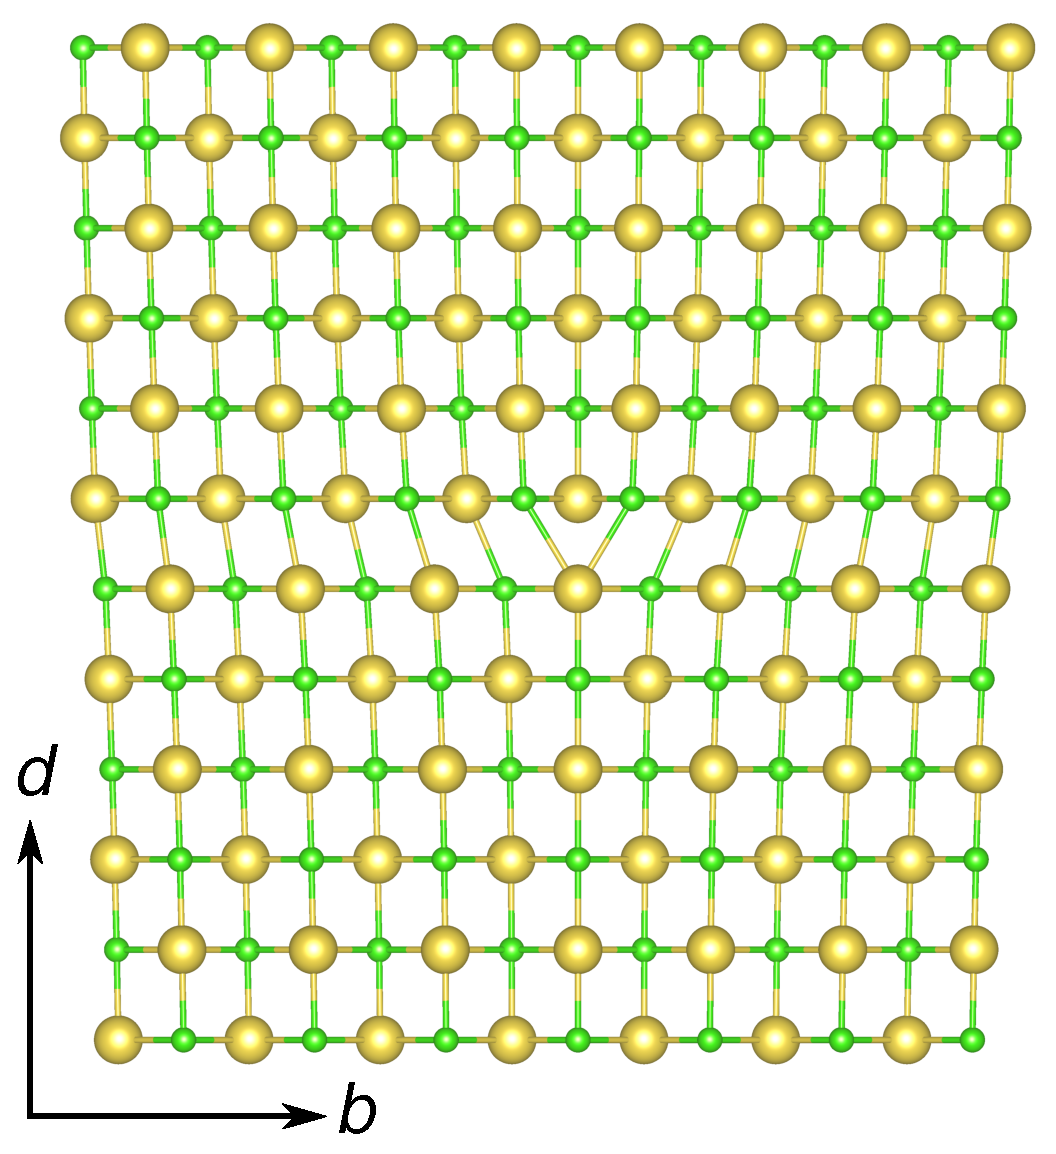
\includegraphics[width=0.6\textwidth]{wide_NaCl}
    \caption{A dislocation with a large width.}
    \end{subfigure}
    ~
    \begin{subfigure}{0.4\textwidth}
    \centering
    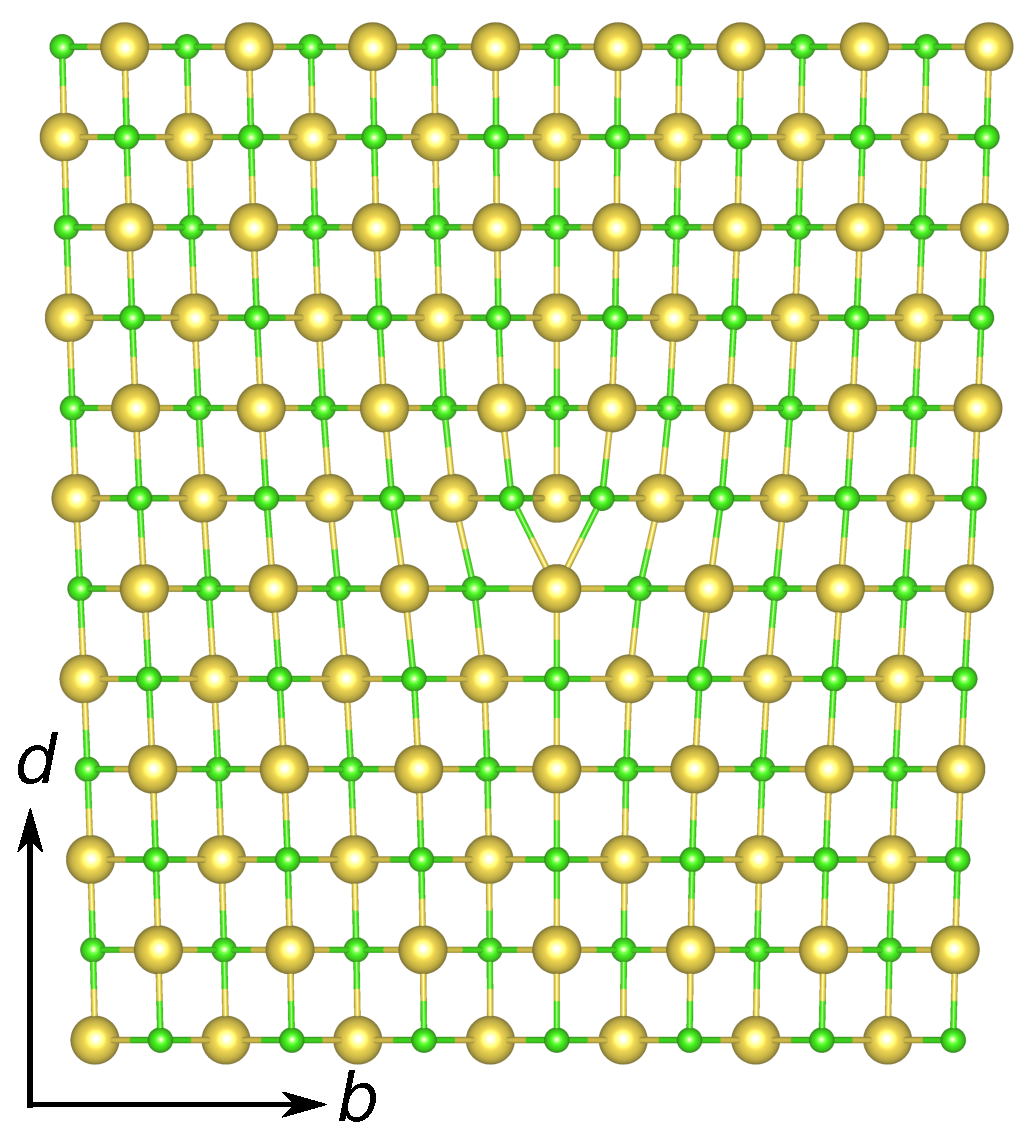
\includegraphics[width=0.6\textwidth]{narrow_NaCl}
    \caption{A dislocation with a small width.}
    \end{subfigure}

	\begin{subfigure}{0.4\textwidth}
	\centering
    \includegraphics[width=0.6\textwidth]{large_c1_NaCl}
    \caption{Large values of $c_1$ and $c_2$.}
	\end{subfigure}
    ~
	\begin{subfigure}{0.4\textwidth}
	\centering
    \includegraphics[width=0.6\textwidth]{large_c3_NaCl}
    \caption{A large value of $c_3$.}
	\end{subfigure}

    \begin{subfigure}{0.8\textwidth}
    \centering
    \includegraphics[width=0.5\textwidth]{typical_NaCl}
    \caption{A ``typical'' configuration.}
    \end{subfigure}

\caption{Various configurations of sodium chloride <110>\{001\} dislocations demonstrating the effects of the parameters of the displacement field defined in \autoref{eqn:displacements}, $w$, $c_1$, $c_2$ and $c_3$. Typical parameters are taken to be those predicted for an isotropic elastic material as given in  Equations~\ref{eqn:half_width} and \ref{eqn:disloc_params}. To illustrate $c_1$, $c_2$ and $c_3$ a ``typical'' value of $w=$~\SI{1.03}{\angstrom} was used, assuming $\nu =$~\num{0.207} \cite{Theocaris1994}.\label{fig:parameters_of_the_disloc_configuration}}
\end{figure}


This provides a parametrised displacement field for a general material in which the width, $w$, and the constants, $c_1$, $c_2$ and $c_3$ are allowed to vary. The width of the dislocation still defines the region with large disregistries (or equivalently small displacements), while $c_1$ and $c_2$ define the magnitude of displacements associated with shear strains around the dislocation core and $c_3$ defines the bending of a crystal that must arise from the introduction of an extra half plane.
To illustrate the displacements produced by these different terms some exaggerated dislocation configurations are shown in \autoref{fig:parameters_of_the_disloc_configuration}.





A final note on the parametrisation of the dislocation structure is that the values $c_1$, $c_2$ and $c_3$ are not constrained, while they have expected signs and magnitudes based on the purely isotropic elastic results described above there is no physical reason they cannot be negative however a negative value of the width reintroduces the discontinuity at which displacements would diverge (in fact it would introduce two, one in each half crystal) which cannot be the case. Hence the constraint that $w>0$ is applied, but $c_1$, $c_2$ and $c_3$ are allowed to vary freely.





